\subsection{Tipologie di convergenze}
Vogliamo stabilire se $f_n:X\to \overline{\mathbb R}$, misurabile $\forall n\in \mathbb N$ converge a $f$ per $n\to +\infty$.
\subsubsection{(def) Pointwise convergence}
$$f_n(x)\to f(x)\quad \forall x\in X$$
\subsubsection{(def) Uniform convergence}
$$\sup_X |f_n-f|\to 0$$
\subsubsection{(def) a.e. convergence}
$$f_n(x)\to f(x) \quad \text{for a.e. }x\in X$$
\subsubsection{(def) $L^\infty$-convergence}
$$\esssup_X|f_n-f|\to 0$$
\subsubsection{(def) $L^1$-convergence}
$$\int_X|f_n-f|\mathrm d\mu\to 0$$
\subsubsection{(def) convergence in measure}
$$\forall \alpha>0\quad \mu(\{ x:|f_n-f|\geq \alpha\})\to 0$$
\subsection{Relations between convergences}
\begin{figure}[h]
    \centering
    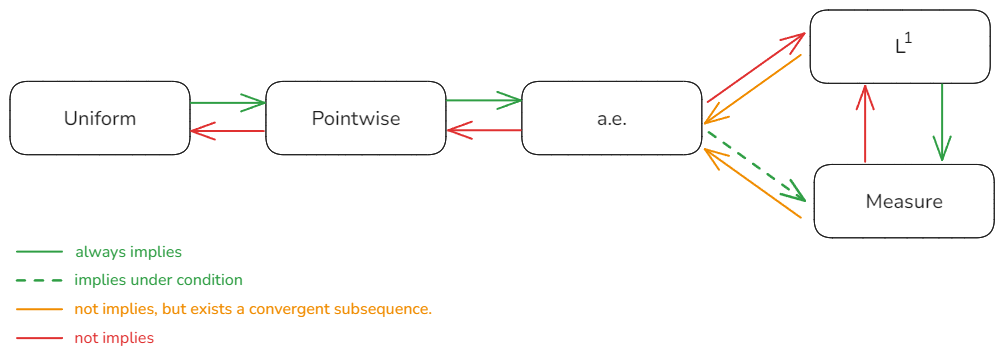
\includegraphics[width=0.9\linewidth]{assets/convergences_image.png}
    \caption{Convergences relations schema}
    \label{fig:enter-label}
\end{figure}
\begin{itemize}
    \item pointwise convergence $\implies$ a.e. convergence
    \item uniform convergence $\implies$ pointwise convergence
    \item uniform convergence $\implies$ $L^\infty$ convergence
\end{itemize}
\subsubsection{(thm) a.e convergence vs convergence in measure}
Let $\mu(X)<+\infty,\ \{f_n\}_n,\ f$ misurabili e a.e. finite in $X$ ($\vert f\vert<+\infty $ a.e. in $X$ e $\vert f_n\vert<+\infty $ a.e. in $X\quad \forall n$).
$$f_n\to f\text{ a.e. in }X\implies f_n\to f\text{ in measure}$$
\subsubsection{(rkm) Typewriter sequence}
We can see that convergence in measure does not imply a.e. convergence.

\subsubsection{(thm) Convergence in measure implies subsequence a.e. convergence}
Given:
\begin{itemize}
    \item $f_n,\ f$ measurable, a.e. finite
\end{itemize}
If $f_n\to f$ in measure, then $\exists \{f_{n_k}\}_{k\in \mathbb N}$ t.c. $f_{n_k}\to f$ a.e. as $k\to+\infty$\\\\
($\{f_{n_k}\}_{k\in \mathbb N}$ è una sottosequenza di $\{f_n\}_n$)

\subsubsection{(thm) $L^1$ convergence vs convergence in measure (*)}
$f_n,\ f\in L^1(X,\mathcal M,\mu)$ \\
$$f_n\to f\text{ in }L^1,\text{ allora }f_n\to f\text{ in measure}$$
\subsubsection{$L^1$ vs a.e. convergence}
In generale, non sono correlati, ma:
\begin{itemize}
    \item Dominated convergence
    $$\begin{cases}f_n\xrightarrow[]{a.e.} f\\ \exists g\in L^1\quad s.t.\quad |f_n|\leq g \quad a.e.\end{cases}\implies f_n\xrightarrow[]{L^1} f$$
    \item Reverse dominated convergence
    $$f_n\xrightarrow[]{L^1}f \implies \exists \text{ subseq }\{ f_{n_k}\}_k\ :\  \begin{cases}
        f_{n_k}\xrightarrow[]{a.e.}f\\
        \exists g\in L^1\ :\ |f_{n_k}|\leq g\quad a.e.
    \end{cases}$$
\end{itemize}
